
\section{Wording Ideas}
\subsection{Explaining the plots}
\begin{itemize}
    \item \quoted{Figure shows the polarized intensity in colorscale overlad with polarization vectors} \cite{Kataoka_2017}
    \item \quoted{Shows the polarization fraction in colorscale} \cite{Kataoka_2017}
\end{itemize}


\subsection{Explaining what we see in the plots}
\begin{itemize}
   \item \quoted{We sucessfully detect the ring-like polarized emission at X mm} \cite{Kataoka_2017}
\end{itemize}
\subsection{Stream/Jet}

\subsection{POLI}
\begin{itemize}
    \item \quoted{The polarized intensity has a peak of X, which corresponds to a $\sigma$ detection with the rms of X}
    \cite{Kataoka_2017}
    \item \quoted{The peak of the polarized intensity is not located at the central star, but on the ring} \cite{Kataoka_2017}
    \item \quoted{The polarized intensity at the location of the central star is lower than the other regions. We interpret this structure as a beam dialution of the central region where polariation is expecte to be azimuthal and thus cancels out each other} \cite{Kataoka_2017}
\end{itemize}





\section{Other Info}
\subsection{Quotes}
\begin{itemize}
    \item \quoted{By modeling the total polarization fraction with a single grain population model, the maximum grain size is constrained t be X \micron} \cite{Kataoka_2017}
\end{itemize}


\section{Why We Care About Dust Grain Size}
\subsection{Quotes}
\begin{itemize}
    \item \quoted{Observational constraints on grain size are important in understanding the first stage of planet formation. } \cite{Kataoka_2015}
\end{itemize}



\section{\cite{Kataoka_2017} Figure 1}

\subsection{Quotes}
\begin{itemize}
    \item \quoted{Illustrate the dependence of the scattering efficiency on the grain size } \cite{Kataoka_2015}
    \item \quoted{Figure \ref{fig: Kataoka2015Figure1Recreation} shows the absorption an scattering mass opacities of dust grains that make the maximum sizes of 1 and 100 \micron} \cite{Kataoka_2017}
    \item \quoted{The mass opacity is written in units of \cmsq per gram of dust grains} \cite{Kataoka_2015}
    \item \quoted{In the case of \amaxtext = 1 \micron, the scattering opacity (red dashed line) is much less than the absorption (solid red line) at approximately millimeter wavelengths } \cite{Kataoka_2015}
    \item \quoted{For the \amaxtext = 100 \micron case, the scattering opacity is lager than absportion (dashed blue larger than solid blue)} \cite{Kataoka_2015}
    \item \quoted{This implies that the scattering at millimeter wavelengths is efficient if the dust grains are as large as 100 \micron} \cite{Kataoka_2015}
    \item \quoted{This is realized in \ppds because dust grains are believed to have grown to \mmt size } \cite{Kataoka_2015}
\end{itemize}




\begin{figure*}[h]
  \centering
  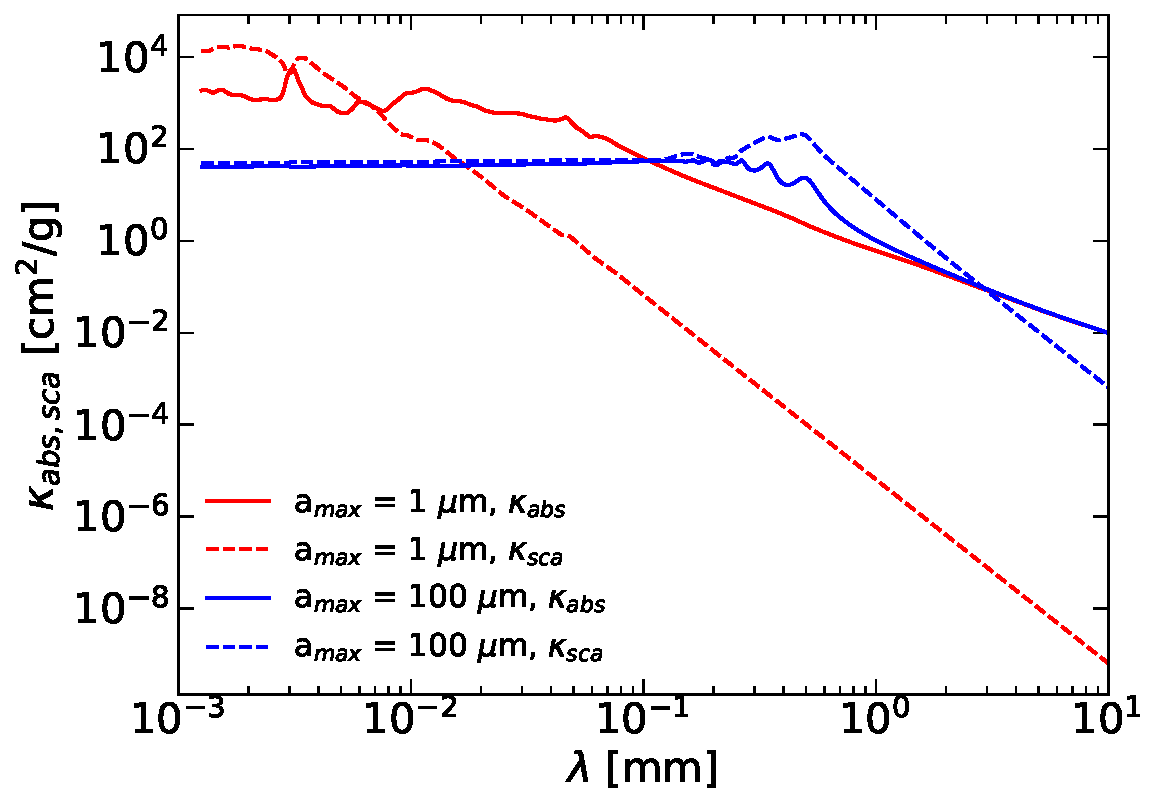
\includegraphics[width=1.1\textwidth]{WRITEUP_AND_IMAGES/IMAGES/WRITEUP/DustModels/Kataoka2015Fig1.pdf}
  \caption{\add{caption}}
  \label{fig: Kataoka2015Figure1Recreation}
\end{figure*}





\section{Polarization Dependence on the Scattering Angle, \cite{Kataoka_2015} Figure 2}

\subsection{Quotes}
\begin{itemize}
    \item \quoted{The \poln by dust scattering strongly depends on its  scattering angle} \cite{Kataoka_2015}
    \item \quoted{Figure \ref{fig: Kataoka2015Figure2Recreation} shows the degree of polarization due to single scatting averaged by the size distribution () for several maximum grain sizes in the cases of two wavelengths } \cite{Kataoka_2017}
\end{itemize}


\begin{figure*}[h]
  \centering
  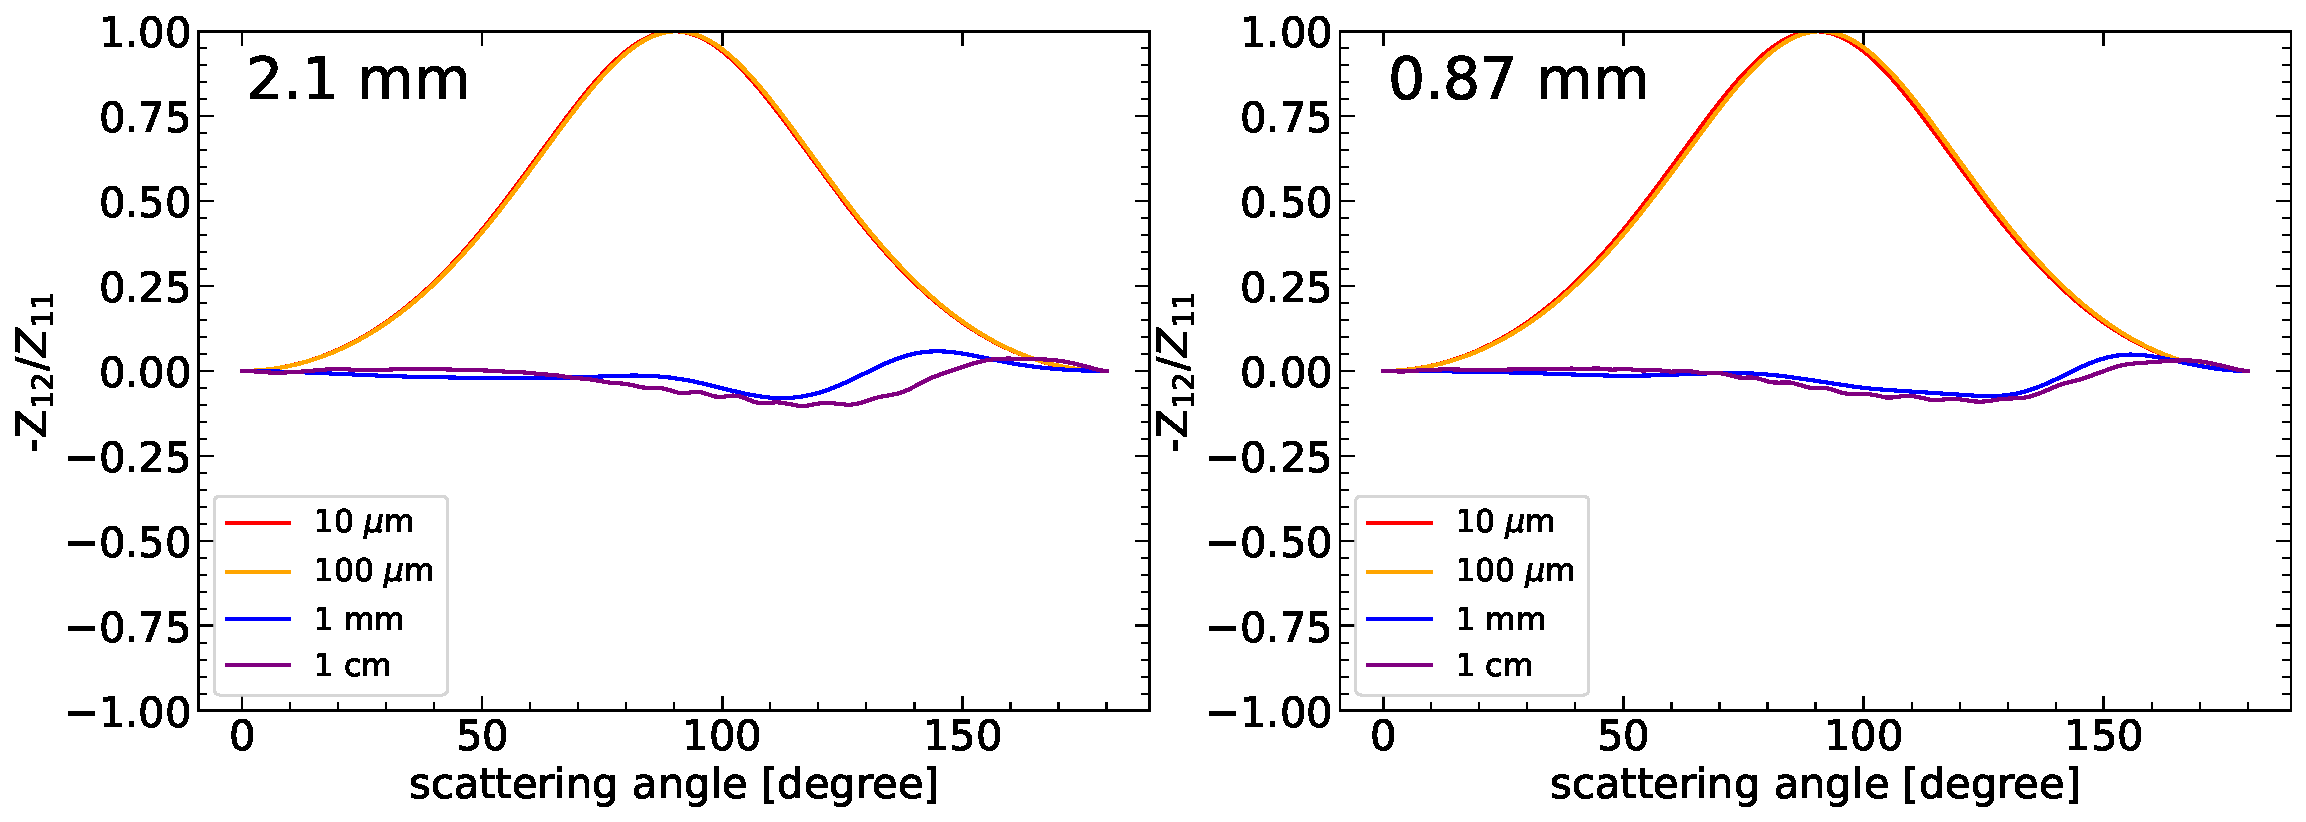
\includegraphics[width=1.1\textwidth]{WRITEUP_AND_IMAGES/IMAGES/WRITEUP/DustModels/Kataoka2015Fig2.pdf}
  \caption{\add{caption}}
  \label{fig: Kataoka2015Figure2Recreation}
\end{figure*}

